\documentclass[varwidth=true, border=2pt]{standalone}
\usepackage{tikz}

\begin{document}
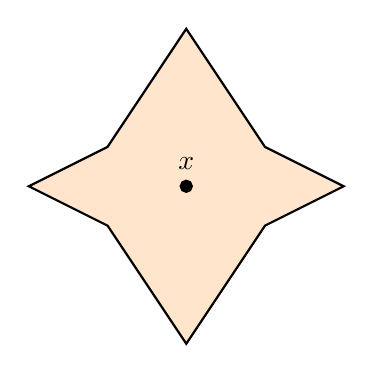
\begin{tikzpicture}[thick]
    \tikzstyle{point}=[circle,thick,draw=black,fill=black,inner sep=0pt,minimum width=4pt,minimum height=4pt]
    \draw[fill=orange!20] (-2,0) -- (-1,0.5) -- (0,2) -- (1,0.5) -- (2,0) -- (1,-0.5) -- (0,-2) -- (-1,-0.5) -- cycle;
    \node (a)[point,label=$x$] at (0,0) {};
\end{tikzpicture}
\end{document}
